\documentclass[
11pt, %The default document font size, options: 10pt, 11pt, 12pt
codirector, % Uncomment to add a codirector to the title page
]{charter} 


% El títulos de la memoria, se usa en la carátula y se puede usar el cualquier lugar del documento con el comando \ttitle
\titulo{Beneficio en el uso de datos privados del buró frente al uso de datos públicos del BCRA para scoring de riesgo crediticio} 


% Nombre del posgrado, se usa en la carátula y se puede usar el cualquier lugar del documento con el comando \degreename
\posgrado{Carrera de Especialización en Inteligencia Artificial}


% Tu nombre, se puede usar el cualquier lugar del documento con el comando \authorname
% IMPORTANTE: no omitir titulaciones ni tildación en los nombres, también se recomienda escribir los nombres completos (tal cual los tienen en su documento)
\autor{Ing. Andrés Montes de Oca}

% El nombre del director y co-director, se puede usar el cualquier lugar del documento con el comando \supname y \cosupname y \pertesupname y \pertecosupname
\director{Paz Llamosas}
\pertenenciaDirector{pertenencia} 
\codirector{Lic. Mg. Erica Grinberg} % para que aparezca en la portada se debe descomentar la opción codirector en los parámetros de documentclass
\pertenenciaCoDirector{UBA}

% Nombre del cliente, quien va a aprobar los resultados del proyecto, se puede usar con el comando \clientename y \empclientename
\cliente{Nombre del cliente}
\empresaCliente{Empresa del cliente}
 
\fechaINICIO{27 de abril de 2026}		%Fecha de inicio de la cursada de GdP \fechaInicioName
\fechaFINALPlan{19 de junio de 2026} 	%Fecha de final de cursada de GdP
\fechaFINALTrabajo{diciembre de 2026}	%Fecha de defensa pública del trabajo final


\begin{document}

\maketitle
\thispagestyle{empty}
\pagebreak


\thispagestyle{empty}
{\setlength{\parskip}{0pt}
\tableofcontents{}
}
\pagebreak


\section*{Registros de cambios}
\label{sec:registro}

\begin{table}[ht]
\label{tab:registro}
\centering
\begin{tabularx}{\linewidth}{@{}|c|X|c|@{}}
\hline
\rowcolor[HTML]{C0C0C0} 
Revisión & \multicolumn{1}{c|}{\cellcolor[HTML]{C0C0C0}Detalles de los cambios realizados} & Fecha      \\ \hline
0      & Creación del documento                                 & \fechaInicioName \\ \hline
1      & Se completa hasta el punto 5 inclusive                 & 10 de mayo de 2026 \\ \hline
2      & Se completa hasta el punto 9 inclusive				  & 17 de mayo de 2026 \\ \hline
%  Se puede agregar algo más \newline
%  En distintas líneas \newline
%  Así                                                    & {día} de {mes} de 202X \\ \hline
%3      & Se completa hasta el punto 12 inclusive                & {día} de {mes} de 202X \\ \hline
%4      & Se completa el plan                                 & {día} de {mes} de 202X \\ \hline

% Si hay más correcciones pasada la versión 4 también se deben especificar acá

\end{tabularx}
\end{table}

\pagebreak



\section*{Acta de constitución del proyecto}
\label{sec:acta}

\begin{flushright}
Buenos Aires, \fechaInicioName
\end{flushright}

\vspace{2cm}

Por medio de la presente se acuerda con el \authorname\hspace{1px} que su Trabajo Final de la \degreename\hspace{1px} se titulará ``\ttitle'' y consistirá en {evaluar la mejora en la predicción de riesgo crediticio al integrar datos de un buró privado frente al uso exclusivo de datos públicos del BCRA}. El trabajo tendrá un presupuesto preliminar estimado de \textcolor{red}{620} horas y un costo estimado de \textcolor{red}{\$ XXX}, con fecha de inicio el \fechaInicioName\hspace{1px} y fecha de presentación pública el \fechaFinalName.

Se adjunta a esta acta la planificación inicial.

\vfill

% Esta parte se construye sola con la información que hayan cargado en el preámbulo del documento y no debe modificarla
\begin{table}[ht]
\centering
\begin{tabular}{ccc}
\begin{tabular}[c]{@{}c@{}}Dr. Ing. Ariel Lutenberg \\ Director posgrado FIUBA\end{tabular} & \hspace{2cm} & \begin{tabular}[c]{@{}c@{}}\clientename \\ \empclientename \end{tabular} \vspace{2.5cm} \\ 
\multicolumn{3}{c}{\begin{tabular}[c]{@{}c@{}} \supname \\ Director del Trabajo Final\end{tabular}} \vspace{2.5cm} \\
\end{tabular}
\end{table}




\section{1. Descripción técnica-conceptual del proyecto a realizar}
\label{sec:descripcion}

En el ámbito de la gestión del riesgo crediticio, la correcta estimación de la probabilidad de default es un pilar fundamental para la sostenibilidad financiera. Tradicionalmente, los modelos de scoring han dependido de datos públicos y transaccionales, como los provistos por la Central de Deudores del Banco Central de la República Argentina (BCRA). Si bien estos datos ofrecen un panorama regulatorio del endeudamiento, suelen carecer de la granularidad necesaria sobre el comportamiento histórico de pago en el ecosistema financiero no regulado y comercial.

El problema analítico central radica en determinar y cuantificar empíricamente si la integración de datos de comportamiento provenientes de burós de crédito privados aporta un valor predictivo incremental que justifique su costo de adquisición. El estado del arte en modelado predictivo indica que la utilización de algoritmos de ensamble (tales como Gradient Boosting o Random Forest) permite maximizar la capacidad de discriminación al capturar interacciones no lineales complejas entre estas múltiples fuentes de datos estructurados.

La propuesta de valor de este proyecto consiste en desarrollar, entrenar y evaluar rigurosamente modelos de machine learning para la clasificación de riesgo, contrastando el desempeño de un modelo base (entrenado exclusivamente con variables públicas del BCRA) contra un modelo extendido (enriquecido con features privadas del buró). La validación metodológica de esta hipótesis se centrará en la evaluación del poder de separación poblacional en distintos segmentos de riesgo, priorizando métricas de discriminación avanzadas, fundamentalmente la mejora porcentual del estadístico Kolmogorov-Smirnov (KS) máximo.

\begin{figure}[htpb]
\centering 
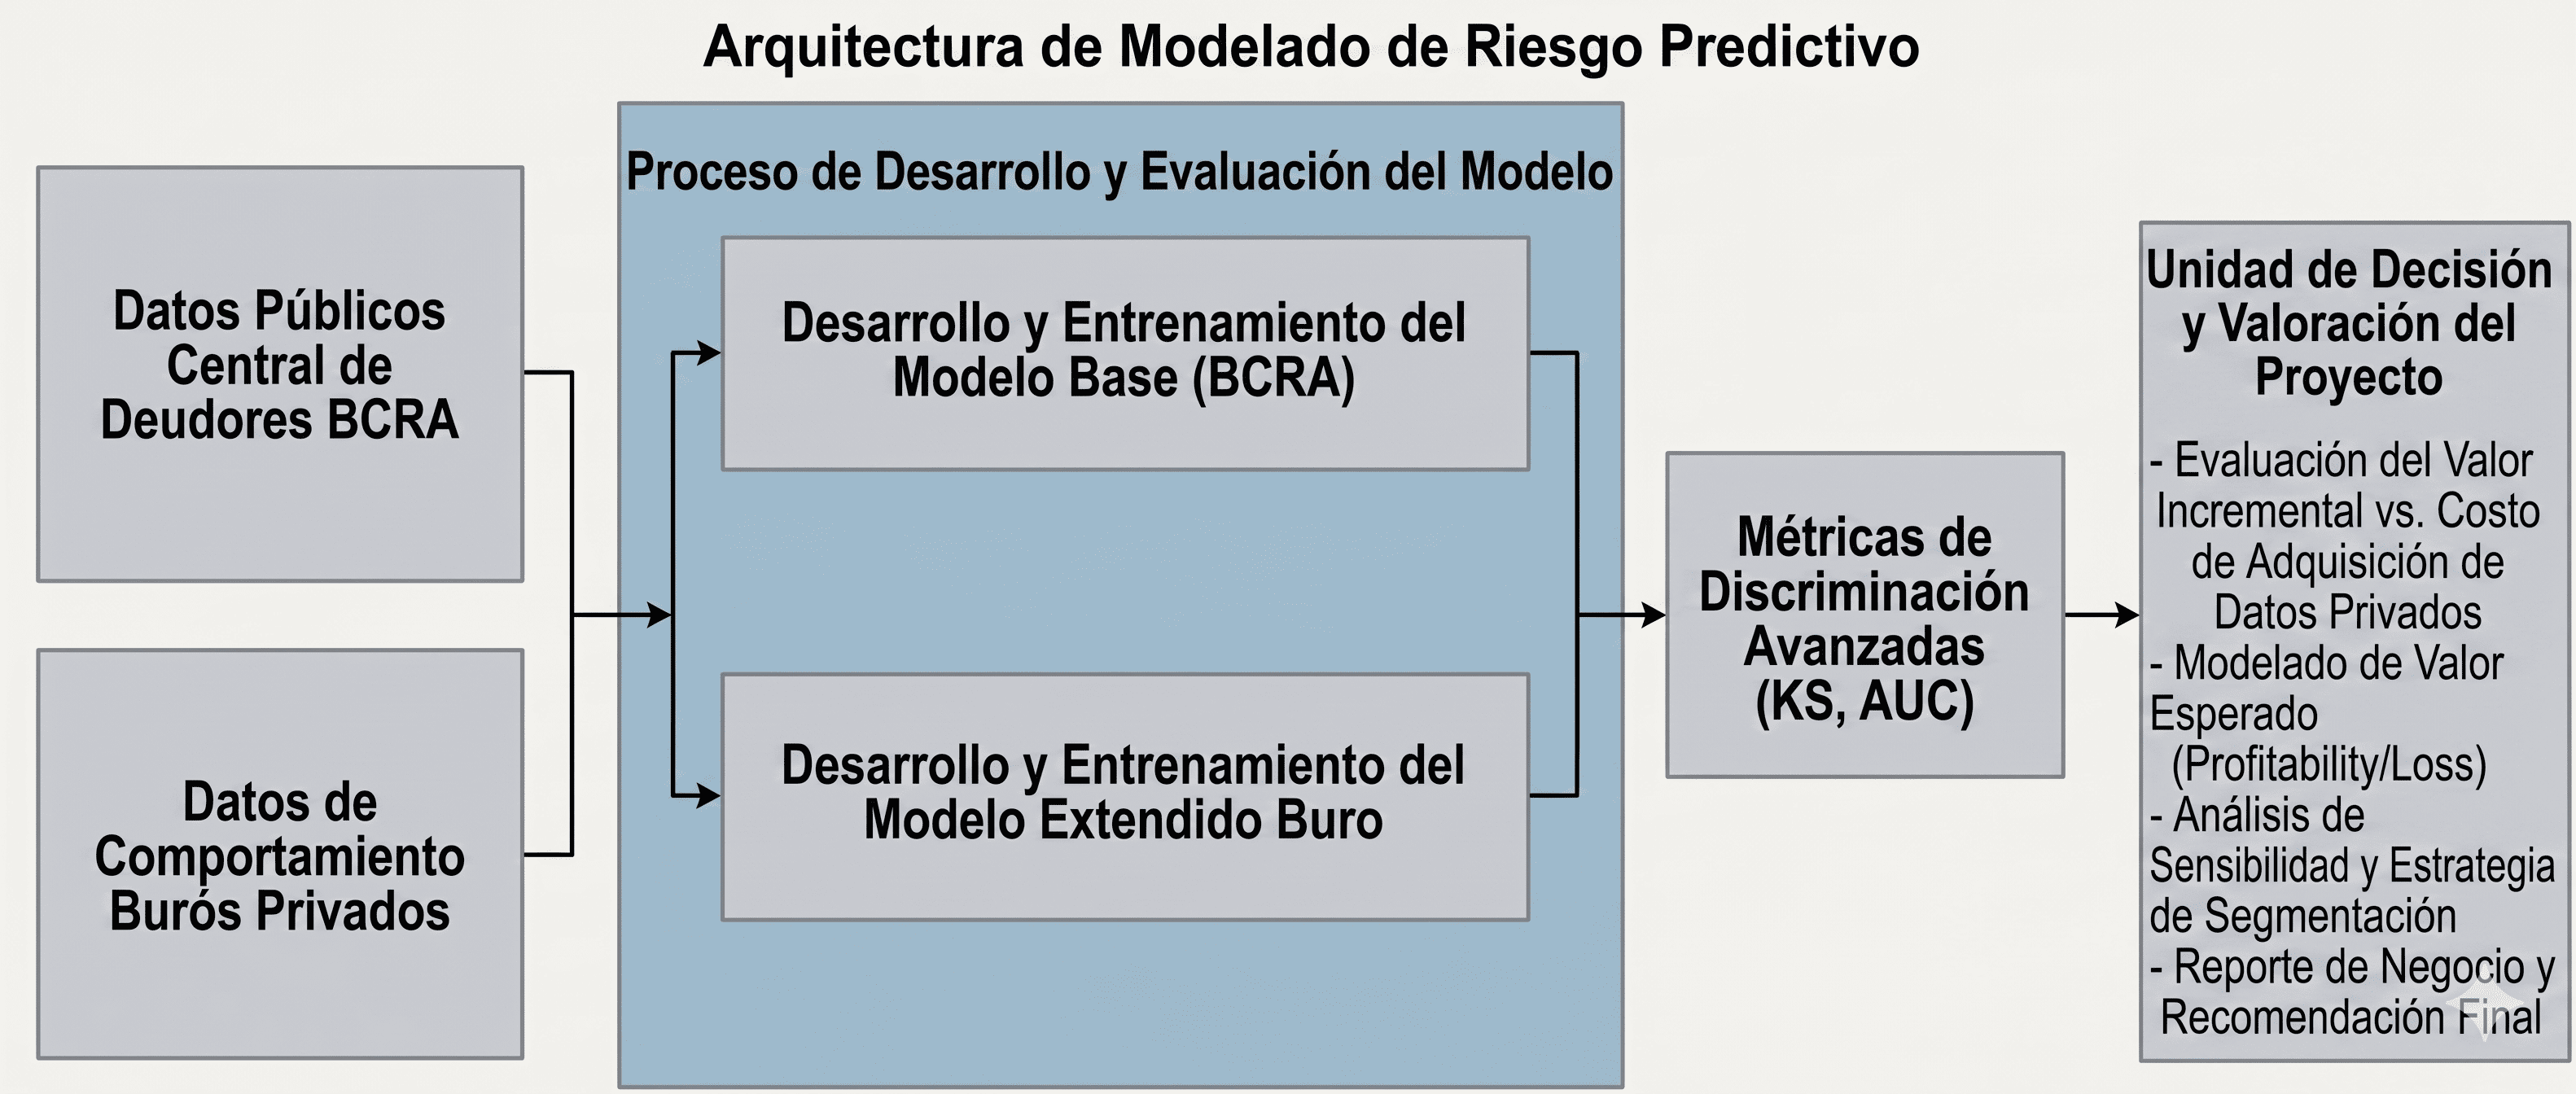
\includegraphics[width=.95\textwidth]{./Figuras/Modelado.png}
\caption{Diagrama en bloques del sistema.}
\label{fig:diagBloques}
\end{figure}

\vspace{25px}


\section{Identificación y análisis de los interesados}
\label{sec:interesados}

En el desarrollo de modelos predictivos de riesgo crediticio, la correcta identificación de los interesados resulta imperativa para garantizar que los requerimientos analíticos y las métricas de \textit{performance} se ajusten a la necesidad real del negocio. La propuesta de valor empírica de este proyecto exige una validación rigurosa por parte de los actores clave para contrastar el valor de la información de comportamiento del buró privado frente a los scores genéricos.

\begin{table}[H]
\caption{Identificación de los interesados}
\label{tab:interesados}
\begin{tabularx}{\linewidth}{@{}|l|X|X|l|@{}}
\hline
\rowcolor[HTML]{C0C0C0}
Rol & Nombre y Apellido & Organización & Puesto \\ \hline
Cliente & John Doe & Nueva Compañía Financiera & Responsable de Riesgo \\ \hline
Responsable & \authorname & FIUBA & Alumno \\ \hline
Orientador & \supname & \pertesupname & Director del Trabajo Final \\ \hline
Opositores & - & Nueva Compañía Financiera & Sector de Finanzas / Presupuesto \\ \hline
\end{tabularx}
\end{table}

A continuación, se detallan las principales características y expectativas metodológicas de cada interesado clave con relación al proyecto:

\begin{itemize}
\item \textbf{Cliente (John Doe):} Es el responsable directo que aprobará los resultados y validará el entregable final. Su evaluación se centrará empíricamente en corroborar si el enriquecimiento algorítmico con datos privados aporta un incremento estadísticamente significativo en la métrica del estadístico Kolmogorov-Smirnov (KS), justificando su viabilidad comercial frente a modelos puramente transaccionales.
\item \textbf{Responsable (\authorname):} Ejerce la autoridad operativa y analítica para gestionar el ciclo de vida del proyecto, abarcando desde la recolección e imputación de variables, hasta la calibración de los hiperparámetros de los algoritmos de ensamble y la contrastación rigurosa de las distribuciones poblacionales.
\item \textbf{Orientador (\supname):} Como experto técnico, supervisará el rigor académico de la experimentación y el diseño algorítmico. Se encargará de asegurar la correcta partición de conjuntos de validación, previniendo sesgos o el sobreajuste (\textit{overfitting}) en la comparación de las fuentes públicas y privadas.
\item \textbf{Opositores (Sector de Finanzas / Presupuesto):} Representan al grupo interno de la entidad cliente que prioriza la reducción de costos operativos a corto plazo. Su oposición radica en considerar el proyecto financieramente oneroso, prefiriendo la utilización exclusiva de datos públicos del BCRA (CENDEU) por ser económicamente más viables, aun asumiendo un detrimento en la \textit{performance} predictiva. El rigor de esta investigación deberá refutar empíricamente su postura, demostrando que la mejora en la capacidad de discriminación (medida a través del KS) compensa holgadamente el costo de adquisición de los datos de buró.
\end{itemize}

\section{3. Propósito del proyecto}
\label{sec:proposito}

Desarrollar y validar empíricamente un modelo predictivo de aprendizaje automático que cuantifique el valor analítico incremental de integrar datos de comportamiento provenientes de un buró de crédito privado frente a la utilización exclusiva de información pública transaccional del BCRA. Este esfuerzo metodológico busca optimizar las políticas de otorgamiento de crédito al maximizar la capacidad de discriminación poblacional, evaluada rigurosamente mediante el estadístico Kolmogorov-Smirnov (KS), proporcionando así la evidencia cuantitativa y objetiva necesaria para justificar económicamente la adquisición de fuentes de datos externas frente a las alternativas genéricas de bajo costo.

\section{4. Alcance del proyecto}
\label{sec:alcance}

El presente proyecto se circunscribe empíricamente al desarrollo, calibración y validación \textit{offline} de modelos predictivos de riesgo crediticio. El esfuerzo analítico se concentrará en cuantificar la mejora de la capacidad de discriminación poblacional, evaluada rigurosamente mediante el estadístico Kolmogorov-Smirnov (KS), al integrar fuentes del buró privado frente a los datos públicos del BCRA.

\textbf{El proyecto incluye taxativamente:}
\begin{itemize}
\item Extracción, depuración y análisis exploratorio exhaustivo de las bases de datos transaccionales públicas (CENDEU) y del buró de crédito privado.
\item Transformación de variables, imputación de valores faltantes e ingeniería de características (\textit{feature engineering}) orientada a capturar el comportamiento financiero.
\item Entrenamiento, optimización de hiperparámetros y validación cruzada utilizando algoritmos de ensamble predictivo.
\item Evaluación metodológica y comparativa del desempeño predictivo entre el modelo base (datos públicos) y el modelo enriquecido (datos privados) segmentando por perfiles de riesgo.
\item Estructuración de los métodos de transformación y modelos de forma tal que sean capaces de ser ejecutados en modalidad \textit{batch} sobre un conjunto de usuarios.
\end{itemize}

\textbf{El proyecto no incluye:}
\begin{itemize}
\item El despliegue o integración (\textit{deployment}) de los modelos algorítmicos en la arquitectura de servidores de producción de la entidad financiera.
\item El desarrollo de una interfaz gráfica de usuario (GUI) o cuadros de mando interactivos para el usuario final.
\item La ejecución del modelo predictivo de clasificación de riesgo en tiempo real (\textit{real-time scoring}).
\item La adquisición o integración de bases de datos de fuentes externas adicionales a las ya provistas para el estudio.
\end{itemize}


\section{5. Supuestos del proyecto}
\label{sec:supuestos}

Para el desarrollo del presente proyecto de investigación empírica se supone que:
\begin{itemize}
\item Se dispondrá de acceso irrestricto, oportuno y continuo a las bases de datos históricas (tanto transaccionales públicas del CENDEU como de comportamiento del buró privado), asumiendo que las mismas poseen la profundidad temporal necesaria para capturar la ciclicidad del riesgo crediticio.
\item Existe una relación matemática subyacente y capturable algorítmicamente entre las variables predictivas históricas seleccionadas y la probabilidad empírica de \textit{default} de los perfiles analizados.
\item Se contará con la infraestructura computacional adecuada (entornos de procesamiento distribuido o máquinas virtuales de alta capacidad) para entrenar, validar y optimizar los hiperparámetros de algoritmos de ensamble complejos sin enfrentar cuellos de botella de memoria.
\item El entorno macroeconómico y el marco normativo del BCRA mantendrán un nivel de estabilidad razonable durante el período de estudio, garantizando que alteraciones exógenas extremas no distorsionen la evaluación comparativa del estadístico Kolmogorov-Smirnov (KS).
\item Se dispondrá del tiempo estipulado en la planificación y la continuidad operativa del Responsable del proyecto para abarcar todas las fases metodológicas del ciclo de vida de los datos, desde la depuración hasta la evaluación final del poder de separación poblacional.
\end{itemize}

\section{6. Requerimientos}
\label{sec:requerimientos}

\begin{enumerate}

    \item \textbf{Requerimientos funcionales}
    \begin{enumerate}
        \item El sistema debe entrenar y evaluar modelos predictivos de riesgo crediticio experimentando con distintos algoritmos, aislando el rendimiento del modelo base (datos públicos del BCRA) respecto al modelo enriquecido (datos privados del buró).
        \item El sistema debe predecir una variable objetivo (\textit{target} o marca de incumplimiento) definida taxativamente como la ocurrencia de un atraso de pago superior a 90 días en el transcurso de los 12 meses posteriores al punto de observación.
        \item El sistema debe calcular y reportar obligatoriamente el estadístico Kolmogorov-Smirnov (KS) como métrica central para evaluar la capacidad del modelo para separar y discriminar las funciones de distribución de dos poblaciones mutuamente excluyentes: los buenos pagadores y los malos pagadores.
        \item El cálculo de variables, la ingeniería de características (\textit{feature engineering}) y la predicción del modelo deben estructurarse para ser ejecutados en modalidad \textit{batch} sobre un conjunto dado de usuarios.
    \end{enumerate}

    \item \textbf{Requerimientos de datos a utilizar}
    \begin{enumerate}
        \item Los datos transaccionales extraídos del buró privado y del BCRA deben abarcar un período histórico definido estrictamente como los 60 meses hacia atrás desde el punto de observación, y procesarse en entornos que garanticen su anonimato y confidencialidad.
        \item Cada usuario debe pertenecer de manera mutuamente excluyente a los conjuntos de entrenamiento, validación o prueba para evitar sesgos analíticos y filtración de información (\textit{data leakage}).
        \item El conjunto de datos crediticios utilizado para entrenar los algoritmos no debe ser compartido públicamente bajo ninguna circunstancia, respetando el marco normativo vigente.
    \end{enumerate}

    \item \textbf{Requerimientos de documentación}
    \begin{enumerate}
        \item Se debe redactar una memoria técnica detallando la optimización de hiperparámetros y el análisis exploratorio realizado sobre los conjuntos de datos.
        \item Se debe elaborar un informe que demuestre empíricamente el incremento porcentual del estadístico KS, justificando de manera cuantitativa la capacidad predictiva de los datos privados del buró frente al modelo base del BCRA.
        \item Se debe analizar y documentar la importancia predictiva de las variables independientes (\textit{feature importance}) para garantizar la explicabilidad y transparencia del \textit{scoring} crediticio.
    \end{enumerate}

\end{enumerate}

\section{7. Historias de usuarios (\textit{Product backlog})}
\label{sec:backlog}

Para la ponderación de las historias de usuario se utilizarán tres criterios, cada uno con tres niveles posibles de calificación:

\textbf{Dificultad}
\begin{itemize}
    \item Baja: 1 punto
    \item Media: 3 puntos
    \item Alta: 5 puntos
\end{itemize}

\textbf{Complejidad}
\begin{itemize}
    \item Baja: 2 puntos
    \item Media: 5 puntos
    \item Alta: 7 puntos
\end{itemize}

\textbf{Incertidumbre}
\begin{itemize}
    \item Baja: 1 punto
    \item Media: 5 puntos
    \item Alta: 10 puntos
\end{itemize}

El puntaje final de cada historia de usuario será calculado como el número de la secuencia de Fibonacci más próximo mayor o igual a la suma de las calificaciones en los 3 criterios. A continuación, se detallan las historias agrupadas analíticamente por rol:

\textbf{Rol: Científico de Datos}
\begin{enumerate}
    \item Como Científico de Datos quiero entrenar un modelo base con información pública del BCRA y un modelo enriquecido con información del buró privado para aislar y cuantificar el incremento del estadístico KS en la separación de buenos y malos pagadores. (5+7+5 = 17 $\rightarrow$ 21 puntos)
    
    \item Como Científico de Datos quiero ejecutar una validación cruzada en diferentes ventanas temporales (\textit{Out-of-Time validation}) para asegurar que la estabilidad de las métricas de separación poblacional se mantenga constante y no sufra volatilidad a causa del sobreajuste algorítmico. (3+7+5 = 15 $\rightarrow$ 21 puntos)
\end{enumerate}

\textbf{Rol: Analista de Riesgos}
\begin{enumerate}\setcounter{enumi}{2}
    \item Como Analista de Riesgos quiero comparar empíricamente la capacidad de discriminación de ambos modelos a través de todos los deciles de riesgo, validando la consistencia predictiva en toda la distribución poblacional para justificar cuantitativamente la adquisición de datos de comportamiento no regulado. (3+5+5 = 13 $\rightarrow$ 13 puntos)
    
    \item Como Analista de Riesgos quiero evaluar la importancia de las variables independientes (\textit{feature importance}) del modelo híbrido para comprender qué características del buró privado determinan el comportamiento crediticio y garantizar la interpretabilidad de la decisión algorítmica. (3+5+1 = 9 $\rightarrow$ 13 puntos)
    
    \item Como Analista de Riesgos quiero calcular el Índice de Estabilidad Poblacional (PSI) de las variables estructuradas del buró privado para garantizar que las distribuciones no sufran deriva de datos (\textit{Data Drift}) temporal frente a la muestra base, asegurando la robustez y vigencia del modelo. (3+5+1 = 9 $\rightarrow$ 13 puntos)
\end{enumerate}

\textbf{Rol: Sector de Finanzas}
\begin{enumerate}\setcounter{enumi}{5}
    \item Como Analista del Sector de Finanzas quiero evaluar las predicciones del modelo híbrido para aumentar la cantidad de usuarios aprobados manteniendo el mismo porcentaje de malos pagadores de la cartera actual (\textit{estrategia de swap-in}), demostrando así la viabilidad comercial y operativa de la información externa. (3+5+1 = 9 $\rightarrow$ 13 puntos)
\end{enumerate}

\textbf{Rol: Gobernanza de Datos}
\begin{enumerate}\setcounter{enumi}{6}
    \item Como Responsable del área de Gobernanza de Datos quiero validar los \textit{pipelines} de preprocesamiento de características transaccionales para asegurar la anonimización de la información privada, certificando el cumplimiento de la Ley 25.326 de Protección de Datos Personales. (1+2+5 = 8 $\rightarrow$ 8 puntos)
\end{enumerate}

\section{8. Entregables principales del proyecto}
\label{sec:entregables}

Los entregables principales del proyecto son:
\begin{itemize}
    \item Memoria técnica del Trabajo Final, documentando la fundamentación empírica, la ingeniería de características y la justificación matemática del incremento en el estadístico Kolmogorov-Smirnov (KS) entre el modelo base (BCRA) y el modelo híbrido, omitiendo cualquier exposición de datos sensibles.
    \item Informe ejecutivo orientado al Sector de Finanzas, detallando de forma clara y directa el beneficio comercial del proyecto. Este documento demostrará empíricamente cómo el uso de los datos del buró permite aumentar la cantidad de usuarios aprobados manteniendo constante el porcentaje de malos pagadores en la cartera.
    \item \textit{Jupyter Notebooks} y \textit{pipeline} de procesamiento de datos. El código fuente no será entregado bajo ningún formato; por políticas de confidencialidad, únicamente estará disponible de forma exclusiva en un repositorio institucional privado.
\end{itemize}

\section{9. Desglose del trabajo en tareas}
\label{sec:wbs}

A continuación se detalla la Estructura de Desglose del Trabajo (EDT/WBS), donde cada paquete de trabajo ha sido descompuesto en tareas técnicas de duración no mayor a 40 horas para garantizar un seguimiento riguroso. El esfuerzo total estimado para este proyecto de modelado predictivo es de 620 horas.

\begin{enumerate}

    \item \textbf{Estudio de la temática y marco normativo (100 h)}
    \begin{enumerate}
        \item Lectura de bibliografía sobre modelos de ensamble aplicados a \textit{scoring} crediticio (40 h).
        \item Relevamiento del marco normativo (Ley 25.326) y pautas de gobernanza de datos para el anonimato (20 h).
        \item Exploración documental de la estructura de diccionarios de variables del BCRA (CENDEU) y del buró privado (40 h).
    \end{enumerate}

    \item \textbf{Definición de lineamientos del modelo (70 h)}
    \begin{enumerate}
        \item Formulación metodológica para la evaluación de la separación poblacional y umbrales del estadístico KS (40 h).
        \item Validación y ajuste de la propuesta analítica y métricas de éxito con el Sector de Finanzas (30 h).
    \end{enumerate}

    \item \textbf{Obtención y preprocesamiento de datos (140 h)}
    \begin{enumerate}
        \item Desarrollo de la consulta estructurada para la extracción de la ventana de observación histórica de 60 meses (40 h).
        \item Integración de los datos tabulares públicos (BCRA) con los datos externos (buró privado) garantizando anonimato (40 h).
        \item Definición y etiquetado de la variable objetivo (\textit{target}): atraso mayor a 90 días en la ventana de desempeño de 12 meses (30 h).
        \item Limpieza exhaustiva de la muestra, tratamiento de valores nulos y filtrado de \textit{outliers} (30 h).
    \end{enumerate}

    \item \textbf{Desarrollo algorítmico y evaluación (210 h)}
    \begin{enumerate}
        \item Análisis exploratorio de datos (EDA) y cálculo de la divergencia de distribuciones (30 h).
        \item Ingeniería de características (\textit{feature engineering}) y selección iterativa de variables predictivas (40 h).
        \item Partición de la muestra y entrenamiento secuencial del modelo base y el modelo enriquecido (40 h).
        \item Cálculo del Índice de Estabilidad Poblacional (PSI) y evaluación del peso predictivo de variables (\textit{feature importance}) (30 h).
        \item Cálculo y análisis comparativo del incremento del estadístico Kolmogorov-Smirnov (KS) en todos los deciles de riesgo (40 h).
        \item Armado del \textit{pipeline} definitivo para la productivización \textit{batch} y estimación de viabilidad comercial (\textit{swap-in}) (30 h).
    \end{enumerate}

    \item \textbf{Documentación y cierre del proyecto (100 h)}
    \begin{enumerate}
        \item Redacción de la memoria técnica documentando la experimentación empírica (60 h).
        \item Elaboración del informe ejecutivo analítico orientado al área de presupuesto y finanzas (20 h).
        \item Preparación del material audiovisual y simulacro para la defensa pública del trabajo (20 h).
    \end{enumerate}

\end{enumerate}

\section{10. Planificación de Sprints}

Organizar las tareas técnicas del proyecto en sprints de trabajo que permitan distribuir de forma equilibrada la carga horaria total, estimada en 600 horas.

\textbf{Consigna:}
\begin{itemize}
  \item Completar una tabla que relacione sprints con HU y tareas técnicas correspondientes.
  \item Incluir estimación en horas para cada tarea.
  \item Indicar responsable y porcentaje de avance estimado o completado.
  \item Contemplar también tareas de planificación, documentación, redacción de memoria y preparación de defensa.
\end{itemize}

\textbf{Conceptos clave:}
\begin{itemize}
  \item Una \'{e}pica es una unidad funcional amplia; una historia de usuario es una funcionalidad concreta; un sprint es una unidad de tiempo donde se ejecutan tareas.
  \item Las tareas son el nivel más desagregado: permiten estimar tiempos, asignar responsables y monitorear progreso.
\end{itemize}

\textbf{Duración sugerida:}
\begin{itemize}
  \item Para un proyecto de 600 h, se recomienda planificar entre 10 y 12 sprints de aproximadamente 2 semanas cada uno.
  \item Asignar entre 45 y 50 horas efectivas por sprint a tareas técnicas.
  \item Reservar 100 a 120 h para actividades no técnicas (planificación, escritura, reuniones, defensa).
\end{itemize}

\textbf{Importante:}
\begin{itemize}
  \item En proyectos individuales, el responsable suele ser el propio autor.
  \item Aun así, desagregar tareas facilita el seguimiento y mejora continua.
\end{itemize}

\textbf{Conversión opcional de Story Points a horas:}
\begin{itemize}
  \item 1 SP \(\approx\) 2 h como referencia flexible.
  \item Tener en cuenta aproximaciones tipo Fibonacci.
\end{itemize}

\begin{table}[htpb]
\centering
\caption{Formato sugerido}
\begin{tabularx}{\linewidth}{@{}|l|l|X|c|l|c|@{}}
\hline
\rowcolor[HTML]{C0C0C0}
Sprint & HU o fase & Tarea & Horas / SP & Responsable & \% Completado \\ \hline
Sprint 0 & Planificación & Definir alcance y cronograma & 10 h & Alumno & 100\% \\ \hline
Sprint 0 & Planificación & Reunión con el tutor/cliente & 5 h & Alumno & 50\% \\ \hline
Sprint 0 & Planificación & Ajuste de los entregables & 6 h & Alumno & 25\% \\ \hline
Sprint 1 & HU1 & Tarea 1 HU1 & 6 h / 3 SP & Alumno & 0\% \\ \hline
Sprint 1 & HU1 & Tarea 2 HU1 & 10 h / 5 SP & Alumno & 0\% \\ \hline
Sprint 2 & HU2 & Tarea 1 HU2 & 7 h / 5 SP & Alumno & 0\% \\ \hline
... & ... & ... & ... & ... & ... \\ \hline
Sprint 5 & Escritura & Redacción memoria & 50 h / 34 SP & Alumno & 0\% \\ \hline
Sprint 6 & Defensa & Preparación de la exposición & 20 h / 13 SP & Alumno & 0\% \\ \hline
\end{tabularx}
\end{table}

\textbf{Recomendaciones:}
\begin{itemize}
  \item Verificar que la carga horaria por sprint sea equilibrada.
  \item Usar sprints de 1 a 3 semanas, acordes al cronograma general.
  \item Actualizar el \% completado durante el seguimiento del proyecto.
  \item Considerar un sprint final exclusivo para pruebas, revisión y ajustes antes de la defensa.
\end{itemize}


\section{11. Diagrama de Gantt (sprints)}
\label{sec:gantt}

Visualizar en un diagrama de Gantt la planificación temporal del proyecto, tomando como base los sprints definidos en la sección anterior. Debe contemplar todas las horas del proyecto.

Consigna:

\begin{itemize}

\item Elaborar un diagrama de Gantt que muestre la secuencia temporal de los sprints.

\item Cada fila debe representar un sprint (con su número o nombre), y el eje horizontal debe indicar el tiempo (en semanas o fechas concretas).

\item Las tareas técnicas derivadas de HU deben diferenciarse visualmente (por ejemplo, con un color distinto) de las tareas no técnicas (planificación, redacción, defensa).

\item Incluir todas las tareas estimadas en cada sprint.
\end{itemize}

Recomendaciones para el Gantt:

\begin{itemize}

	\item Podés usar herramientas gratuitas como TeamGantt, ClickUp, GanttProject, [Google Sheets], [Trello + Planyway], entre otras.
	\item Ordená los sprints de forma cronológica, comenzando con Sprint 0 (planificación) y finalizando con el sprint de defensa.
	\item Asegurate de reflejar la duración realista de cada sprint según tu disponibilidad y el cronograma general del posgrado.
	\item Incluí hitos importantes: reuniones, entregas parciales, defensa.
\end{itemize}


Incluir una imagen legible del diagrama de Gantt. Si es muy ancho, presentar primero la tabla y luego el gráfico de barras.



\section{12. Gobernanza de datos}
\label{sec:gobernanza}

En esta sección se debe analizar de manera integral el marco normativo y ético asociado al uso de los datos y al desarrollo de soluciones basadas en inteligencia artificial.

El análisis se divide en dos partes:

\begin{itemize}
  \item Cumplimiento normativo.
  \item Ética en el uso de inteligencia artificial.
\end{itemize}

\subsection{Cumplimiento normativo}
Este análisis es clave para garantizar el cumplimiento normativo y evitar conflictos legales durante el desarrollo y publicación del proyecto.

En esta subsección se debe identificar si los datos utilizados en el proyecto están sujetos a normativas de protección de datos y privacidad, y en qué condiciones pueden emplearse.

Aspectos a considerar:

\begin{itemize}
  \item Determinar si los datos están regulados por normativas como el GDPR, la Ley 25.326 de Protección de Datos Personales (Argentina), la HIPAA u otras, según la jurisdicción o la temática del proyecto.
  \item Aclarar si las fuentes de datos son propias, de acceso público o licenciadas. En este último caso, explicitar la licencia correspondiente y sus condiciones de uso. Realizar este mismo análisis para las herramientas y, en caso de corresponder, para los modelos preentrenados a emplear.
  \item Analizar la viabilidad legal del proyecto, considerando los mecanismos necesarios para garantizar el cumplimiento normativo y la trazabilidad de los datos.
\end{itemize}

\subsection{Ética en el uso de inteligencia artificial}

En esta subsección se debe reflexionar sobre los aspectos éticos vinculados al uso de datos y algoritmos de inteligencia artificial. Se espera una evaluación de la integridad del sistema y su impacto social.

Aspectos a considerar:

\begin{itemize}
	\item Identificar posibles sesgos en los datos o modelos (ideológicos, culturales, de género, geográficos, etc.) y analizar sus consecuencias (por ejemplo: discriminación, manipulación, pérdida de privacidad o desinformación).
	\item Analizar los posibles riesgos en términos de impacto social del uso indebido de la solución a desarrollar.
	\item En caso de corresponder, proponer medidas de mitigación y mecanismos de confianza (auditorías, documentación, trazabilidad, revisión humana, etc.).
	\item Finalmente, elaborar una reflexión general sobre la ética del proyecto, considerando tanto la equidad y transparencia del sistema como su impacto potencial en la sociedad.

\end{itemize}


\section{13. Gestión de riesgos}
\label{sec:riesgos}

\begin{consigna}{red}
a) Identificación de los riesgos (al menos cinco) y estimación de sus consecuencias:
 
Riesgo 1: detallar el riesgo (riesgo es algo que si ocurre altera los planes previstos de forma negativa)
\begin{itemize}
	\item Severidad (S): mientras más severo, más alto es el número (usar números del 1 al 10).\\
	Justificar el motivo por el cual se asigna determinado número de severidad (S).
	\item Probabilidad de ocurrencia (O): mientras más probable, más alto es el número (usar del 1 al 10).\\
	Justificar el motivo por el cual se asigna determinado número de (O). 
\end{itemize}   

Riesgo 2:
\begin{itemize}
	\item Severidad (S): X.\\
	Justificación...
	\item Ocurrencia (O): Y.\\
	Justificación...
\end{itemize}

Riesgo 3:
\begin{itemize}
	\item Severidad (S):  X.\\
	Justificación...
	\item Ocurrencia (O): Y.\\
	Justificación...
\end{itemize}


b) Tabla de gestión de riesgos:      (El RPN se calcula como RPN=SxO)

\begin{table}[htpb]
\centering
\begin{tabularx}{\linewidth}{@{}|X|c|c|c|c|c|c|@{}}
\hline
\rowcolor[HTML]{C0C0C0} 
Riesgo & S & O & RPN & S* & O* & RPN* \\ \hline
       &   &   &     &    &    &      \\ \hline
       &   &   &     &    &    &      \\ \hline
       &   &   &     &    &    &      \\ \hline
       &   &   &     &    &    &      \\ \hline
       &   &   &     &    &    &      \\ \hline
\end{tabularx}%
\end{table}

Criterio adoptado: 

Se tomarán medidas de mitigación en los riesgos cuyos números de RPN sean mayores a...

Nota: los valores marcados con (*) en la tabla corresponden luego de haber aplicado la mitigación.

c) Plan de mitigación de los riesgos que originalmente excedían el RPN máximo establecido:
 
Riesgo 1: plan de mitigación (si por el RPN fuera necesario elaborar un plan de mitigación).
  Nueva asignación de S y O, con su respectiva justificación:
  \begin{itemize}
	\item Severidad (S*): mientras más severo, más alto es el número (usar números del 1 al 10).
          Justificar el motivo por el cual se asigna determinado número de severidad (S).
	\item Probabilidad de ocurrencia (O*): mientras más probable, más alto es el número (usar del 1 al 10).
          Justificar el motivo por el cual se asigna determinado número de (O).
	\end{itemize}

Riesgo 2: plan de mitigación (si por el RPN fuera necesario elaborar un plan de mitigación).
 
Riesgo 3: plan de mitigación (si por el RPN fuera necesario elaborar un plan de mitigación).

\end{consigna}

\section{14. Sprint Review}
\label{sec:sprint_review}

La revisión de sprint (\emph{Sprint Review}) es una práctica fundamental en metodologías ágiles. Consiste en revisar y evaluar lo que se ha completado al finalizar un sprint. En esta instancia, se presentan los avances y se verifica si las funcionalidades cumplen con los criterios de aceptación establecidos. También se identifican entregables parciales y se consideran ajustes si es necesario.

Aunque el proyecto aún se encuentre en etapa de planificación, esta sección permite proyectar cómo se evaluarán las funcionalidades más importantes del backlog. Esta mirada anticipada favorece la planificación enfocada en valor y permite reflexionar sobre posibles obstáculos.

\textbf{Objetivo:} anticipar cómo se evaluará el avance del proyecto a medida que se desarrollen las funcionalidades, utilizando como base al menos cuatro historias de usuario del \emph{Product Backlog}.


Seleccionar al menos 4 HU del Product Backlog. Para cada una, completar la siguiente tabla de revisión proyectada:

\textbf{Formato sugerido:}
\begin{table}[htpb]
\renewcommand{\arraystretch}{1.5}
\begin{tabular}{|>{\raggedright\arraybackslash}m{2.4cm}|
                >{\raggedright\arraybackslash}m{2.3cm}|
                >{\raggedright\arraybackslash}m{3cm}|
                >{\raggedright\arraybackslash}m{3cm}|
                >{\raggedright\arraybackslash}m{3cm}|}
\hline
\rowcolor[HTML]{CCCCCC}
\textbf{HU seleccionada} & \textbf{Tareas asociadas} & \textbf{Entregable esperado} & \textbf{¿Cómo sabrás que está cumplida?} & \textbf{Observaciones o riesgos} \\
\hline
                         & Tarea 1 &                             &                                           &                                     \\ \cline{2-2}
\multirow{-2}{=}{HU1}    & Tarea 2 & \multirow{-2}{=}{Módulo funcional} & \multirow{-2}{=}{Cumple criterios de aceptación definidos} & \multirow{-2}{=}{Falta validar con el tutor} \\
\hline
                         & Tarea 1 &                             &                                           &                                     \\ \cline{2-2}
\multirow{-2}{=}{HU3}    & Tarea 2 & \multirow{-2}{=}{Reporte generado} & \multirow{-2}{=}{Exportación disponible y clara} & \multirow{-2}{=}{Requiere datos reales} \\
\hline
                         & Tarea 1 &                             &                                           &                                     \\ \cline{2-2}
\multirow{-2}{=}{HU5}    & Tarea 2 & \multirow{-2}{=}{Panel de gestión} & \multirow{-2}{=}{Roles diferenciados operativos} & \multirow{-2}{=}{Riesgo en integración} \\
\hline
                         & Tarea 1 &                             &                                           &                                     \\ \cline{2-2}
\multirow{-2}{=}{HU7}    & Tarea 2 & \multirow{-2}{=}{Informe trimestral} & \multirow{-2}{=}{PDF con gráficos y evolución} & \multirow{-2}{=}{Puede faltar tiempo para ajustes} \\
\hline
\end{tabular}
\end{table}

\section{15. Sprint Retrospective}    
\label{sec:sprint_retro}

La retrospectiva de sprint es una práctica orientada a la mejora continua. Al finalizar un sprint, el equipo (o el alumno, si trabaja de forma individual) reflexiona sobre lo que funcionó bien, lo que puede mejorarse y qué acciones concretas pueden implementarse para trabajar mejor en el futuro.

Durante la cursada se propuso el uso de la \textbf{Estrella de la Retrospectiva}, que organiza la reflexión en torno a cinco ejes:

\begin{itemize}
\item  ¿Qué hacer más?
\item  ¿Qué hacer menos?
\item  ¿Qué mantener?
\item  ¿Qué empezar a hacer?
\item  ¿Qué dejar de hacer?
\end{itemize}

Aun en una etapa temprana, esta herramienta permite que el alumno planifique su forma de trabajar, identifique anticipadamente posibles dificultades y diseñe estrategias de organización personal.

\textbf{Objetivo:} reflexionar sobre las condiciones iniciales del proyecto, identificando fortalezas, posibles dificultades y estrategias de mejora, incluso antes del inicio del desarrollo.


Completar la siguiente tabla tomando como referencia los cinco ejes de la Estrella de la Retrospectiva (\emph{Starfish} o estrella de mar). Esta instancia te ayudará a definir buenas prácticas desde el inicio y prepararte para enfrentar el trabajo de forma organizada y flexible. Se deberá completar la tabla al menos para 3 sprints técnicos y 1 no técnico.

\textbf{Formato sugerido:}

\begin{table}[htpb]
\renewcommand{\arraystretch}{1.4}
\begin{tabular}{|>{\raggedright\arraybackslash}p{1.8cm}|
                >{\raggedright\arraybackslash}p{2.3cm}|
                >{\raggedright\arraybackslash}p{2.3cm}|
                >{\raggedright\arraybackslash}p{2.3cm}|
                >{\raggedright\arraybackslash}p{2.3cm}|
                >{\raggedright\arraybackslash}p{2.3cm}|}
\hline
\rowcolor[HTML]{CCCCCC} 
\textbf{Sprint tipo y N°} & \textbf{¿Qué hacer más?} & \textbf{¿Qué hacer menos?} & \textbf{¿Qué mantener?} & \textbf{¿Qué empezar a hacer?} & \textbf{¿Qué dejar de hacer?} \\
\hline
Sprint técnico - 1 & Validaciones continuas con el alumno & Cambios sin versión registrada & Pruebas con datos simulados & Documentar cambios propuestos & Ajustes sin análisis de impacto \\
\hline
Sprint técnico - 2 & Verificar configuraciones en múltiples escenarios & Modificar parámetros sin guardar historial & Perfiles reutilizables & Usar logs para configuración & Repetir pruebas manuales innecesarias \\
\hline
Sprint técnico - 8 & Comparar correlaciones con casos previos & Cambiar parámetros sin justificar & Revisión cruzada de métricas & Anotar configuraciones usadas & Trabajar sin respaldo de datos \\
\hline
Sprint no técnico - 12 (por ej.: ``Defensa'') & Ensayos orales con feedback & Cambiar contenidos en la memoria & Material visual claro & Dividir la presentación por bloques & Agregar gráficos difíciles de explicar \\
\hline
\end{tabular}
\end{table}





\end{document}
